\chapter{Six Principles}
\label{ch:principles}

\newcommand{\NineRWsteps}{100}
\newcommand{\NineRWrms}{9.98}
\newcommand{\NineRWwalks}{100\,000}


Astrophysics can look like a long list of formulas. The Jeans mass, the Eddington luminosity, the free-fall time, the Chandrasekhar mass and the Planck spectrum are usually met one at a time, each with its own derivation. The list grows with every new object.

The list does not have to be remembered. Almost every formula about stars and gas comes from six general principles, applied with the classical and quantum physics the reader already knows. Each result is then a short calculation that can be redone whenever the formula itself is forgotten.

\begin{table}[htbp]
	\centering
	\begin{tabular}{@{}l l p{0.62\textwidth}@{}}
		\toprule
		& \textbf{Principle} & \textbf{Statement} \\
		\midrule
		P1 & Conservation & The mass, momentum, energy and angular momentum in a region change only by what flows across its boundary and by the forces that act on it. \\
		P2 & Gravity of a sphere & Inside a spherical body, a parcel at radius $r$ is pulled only by the mass inside $r$, as if it sat at the centre. \\
		P3 & Counting states & Phase space comes in cells of size $h^3$. Pressure, energy density and populations follow from counting the states and how full each one is. \\
		P4 & Balance of rates & In a steady state every gain is matched by a loss. In equilibrium every process is matched by its own reverse. \\
		P5 & Random walk & After $N$ steps in random directions a particle is about $\sqrt N$ steps from its start, so anything that scatters often moves down its own gradient. \\
		P6 & Compare two scales & The ratio of two times or two lengths decides which physics matters. A ratio near one marks a transition. \\
		\bottomrule
	\end{tabular}
	\caption{The six principles.}
	\label{pr:tab:principles}
\end{table}

None of the six is new physics. Each is a familiar law put in the form that applies directly to gas, light and gravity. Each has one general form, written with as few symbols as possible, and every result built on them names the principles it combines.

% ==============================================================================
\section{Conservation (P1)}
\label{pr:sec:p1}

The Kepler problem of Chapter~\ref{ch:twobody} was solved by two conserved quantities. Conservation of the energy and of the angular momentum turned six second-order equations into an orbit that could be written down (Section~\ref{sec:com_separation} onwards).

A star is not two bodies. It holds about $10^{57}$ particles, and nobody can follow each of them.

Think of a water tank in a house. Water comes in through one pipe and leaves through another. To know how much water the tank holds a minute from now, nobody follows single molecules. One watches the two pipes. The water inside changes by what flows in minus what flows out, and nothing that happens inside the tank can change that.

A star can be treated the same way. Take any fixed region inside it. The mass in that region changes only by gas flowing across its boundary. Its momentum changes by the momentum that gas carries across the boundary and by the forces acting on the region. This is conservation written for a fixed region instead of a single particle, principle P1.

The tank in numbers. It holds $200\,\mathrm{L}$, water flows in at $3\,\mathrm{L/min}$ and out at $5\,\mathrm{L/min}$. The volume changes at $3-5=-2\,\mathrm{L/min}$, so the tank is empty after $100$ minutes. Only the two flows were needed.

The picture to keep is a box with arrows crossing its faces. Arrows pointing in add to what is inside, arrows pointing out take away.

The same bookkeeping is the continuity equation for charge in electromagnetism, the probability current in quantum mechanics, and the conservation of energy and angular momentum in Chapter~\ref{ch:twobody}. For stars it gives hydrostatic equilibrium (Chapter~\ref{ch:selfgrav}), the change of light along a ray (Chapter~\ref{ch:radiation}) and the energy equation of a star (Chapter~\ref{ch:structure}). For a gas it gives two equations, one for mass and one for momentum.

\paragraph{Mass.} Let a gas have density $\rho(\vecr,t)$ and velocity $\vec v(\vecr,t)$. Take a fixed volume $V$ with surface $S$, and let $d\vec A$ be an outward-pointing element of $S$. Gas crossing $d\vec A$ carries mass out at the rate $\rho\,\vec v\cdot d\vec A$. The mass inside therefore changes as
\begin{align}
	\dv{t}\int_V \rho\,dV
	&\eqby{1} -\oint_S \rho\,\vec v\cdot d\vec A \nonumber\\
	&\eqby{2} -\int_V \nabla\cdot(\rho\vec v)\,dV .
\end{align}
\begin{explain}
	\item Mass inside changes only by the flow across the surface (P1).
	\item The divergence theorem.
\end{explain}
The volume is fixed, so the time derivative on the left acts only on $\rho$ and can be taken inside the integral. Both sides are then integrals over the same $V$,
\[
\int_V\left[\pdv{\rho}{t}+\nabla\cdot(\rho\vec v)\right]dV = 0 .
\]
This holds for every choice of $V$, however small, so the integrand itself vanishes,
\begin{equation}
	\boxed{\pdv{\rho}{t}+\nabla\cdot(\rho\vec v)=0.}
	\label{pr:eq:continuity}
\end{equation}
This is the \textbf{continuity equation}. It holds for any fluid and says nothing about forces.

\paragraph{Momentum.} The $i$-th component of the momentum inside $V$ is $\int_V\rho v_i\,dV$. It changes in three ways. Gas crossing the surface carries momentum $\rho v_i$ at the rate $\rho v_i\,\vec v\cdot d\vec A$. The pressure $P$ of the surrounding gas pushes inward on each surface element with the force $-P\,d\vec A$. Gravity pulls on every element of mass with the acceleration $\vec g$. Writing the surface element as $dA_j$ and summing over repeated indices,
\begin{align}
	\dv{t}\int_V\rho v_i\,dV
	&\eqby{1} -\oint_S \rho v_iv_j\,dA_j-\oint_S P\,\delta_{ij}\,dA_j+\int_V\rho g_i\,dV \nonumber\\
	&\eqby{2} \int_V\Big[-\partial_j\big(\rho v_iv_j+P\delta_{ij}\big)+\rho g_i\Big]dV .
\end{align}
\begin{explain}
	\item The three ways listed above (P1). The pressure force is written with $\delta_{ij}$ so that both surface terms have the same form.
	\item The divergence theorem, applied to each surface term.
\end{explain}
The quantity being differentiated, $\rho v_iv_j+P\delta_{ij}$, is the flux of the $i$-th component of momentum in direction $j$. It is a $3\times3$ matrix, the \textbf{momentum flux},
\begin{equation}
	\Pi=
	\begin{pmatrix}
		\rho v_x^2+P & \rho v_xv_y & \rho v_xv_z\\
		\rho v_yv_x & \rho v_y^2+P & \rho v_yv_z\\
		\rho v_zv_x & \rho v_zv_y & \rho v_z^2+P
	\end{pmatrix}
	=\rho\,\vec v\,\vec v^{\mathsf T}+P\,\Id.
	\label{pr:eq:momentum_flux}
\end{equation}
The first part is momentum carried by the bulk flow. The second part, $P$ on the diagonal, is momentum carried across the surface by the random motion of the particles, which is what pressure is (Section~\ref{pr:sec:p3}). Removing the integrals as for the mass, and using $\Pi$,
\begin{equation}
	\pdv{(\rho v_i)}{t}+\partial_j\Pi_{ij}=\rho g_i .
	\label{pr:eq:momentum_conservative}
\end{equation}
The left side can be simplified with the continuity equation. Writing $\Pi_{ij}=\rho v_iv_j+P\delta_{ij}$,
\begin{align}
	\pdv{(\rho v_i)}{t}+\partial_j(\rho v_iv_j)
	&\eqby{1} v_i\left[\pdv{\rho}{t}+\partial_j(\rho v_j)\right]+\rho\left[\pdv{v_i}{t}+v_j\,\partial_jv_i\right] \nonumber\\
	&\eqby{2} \rho\left[\pdv{v_i}{t}+v_j\,\partial_jv_i\right].
\end{align}
\begin{explain}
	\item The product rule, applied to $\rho v_i$ and to $\rho v_j\cdot v_i$.
	\item The first bracket is the continuity equation \eqref{pr:eq:continuity}, so it vanishes.
\end{explain}
With $\partial_j(P\delta_{ij})=\partial_iP$, Eq.~\eqref{pr:eq:momentum_conservative} becomes the \textbf{Euler equation},
\begin{equation}
	\boxed{\rho\left(\pdv{\vec v}{t}+(\vec v\cdot\nabla)\vec v\right)=-\nabla P+\rho\,\vec g.}
	\label{pr:eq:euler}
\end{equation}
The left side is mass times the acceleration of a parcel that moves with the gas. The right side is the force on it. Pressure acts only through its gradient, since a uniform pressure pushes equally on all sides of a parcel. The gravity $\vec g$ comes from P2 and the pressure from P3.

\paragraph{Counting unknowns.} The unknowns are $\rho$, the three components of $\vec v$, and $P$, five in all. The equations are continuity and the three components of Euler, four in all. One relation is missing. It is the equation of state, which gives $P$ from the density and the temperature (P3). The temperature is then a sixth unknown, and the sixth equation is conservation of energy, written for a star in Section~\ref{st:sec:four_equations}. This is the same count of unknowns against equations that fixed the twelve constants of the two-body problem.

\paragraph{Angular momentum.} When gravity is the only force and it points to a fixed centre, $\vec g\parallel\rhat$, each parcel keeps its angular momentum per unit mass $\vecr\times\vec v$. Following a parcel,
\[
\dv{t}\big(\vecr\times\vec v\big)=\vec v\times\vec v+\vecr\times\dv{\vec v}{t}=\vecr\times\vec g=0,
\]
exactly as for the single body of Eq.~\eqref{eq:kepler2}. With pressure present, neighbouring parcels can trade angular momentum through pressure forces, but the internal forces come in equal and opposite pairs, so the total angular momentum of an isolated cloud does not change. This is what turns a collapsing cloud into a disk (Section~\ref{sg:sec:rotation}).

% ==============================================================================
\section{Gravity of a Sphere (P2)}
\label{pr:sec:p2}

Newton's law of gravity between two points, $GMm/r^2$, ran the whole of Chapter~\ref{ch:twobody}.

A star or a gas cloud is not a point. Every bit of it pulls on every other bit, and adding all those pulls one by one looks hopeless.

Imagine a well dug straight down to the centre of the Earth, and suppose for now that the Earth has the same density everywhere. At the surface you have your usual weight. Halfway down you weigh half as much. The rock above your head forms a shell around you, and the pulls from its different sides cancel exactly. Only the ball of rock below you counts, and it is smaller.

Inside a spherical star the same is true. A parcel of gas at radius $r$ feels only the mass inside $r$, and feels it as if that mass sat at the centre. Everything outside $r$, however it is arranged in shells, pulls with zero net force. That is principle P2.

The well in numbers. For the uniform Earth the mass inside radius $r$ is $M(r/R)^3$, so the pull is
\[
g(r)=\frac{G\,M(r/R)^3}{r^2}=\frac{GM}{R^2}\,\frac rR ,
\]
which falls linearly to zero at the centre. Halfway down, at $r=R/2$, it is $9.8/2=4.9\,\mathrm{m\,s^{-2}}$.

The picture is Figure~\ref{pr:fig:shell_gauss}. Draw a sphere of radius $r$ through the parcel. The mass inside it sets the pull, and the shell outside it does nothing.

\begin{figure}[htbp]
	\centering
	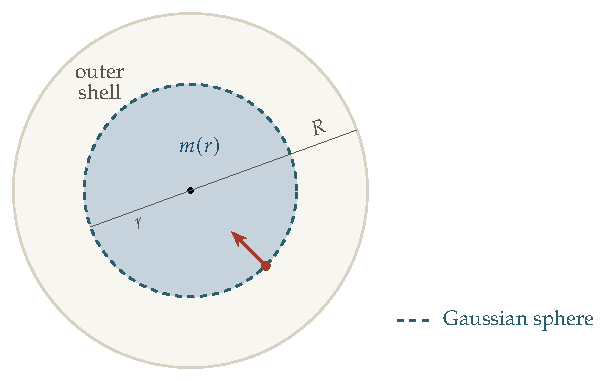
\includegraphics{fig_ch9_shell_gauss.pdf}
	\caption{A spherical star of radius $R$. The dashed sphere of radius $r$ passes through a parcel (dot), which is pulled toward the centre (arrow). The shaded ball holds the mass $m(r)$. The outer shell lies between $r$ and $R$.}
	\label{pr:fig:shell_gauss}
\end{figure}

The same law with charge in place of mass is Gauss's law of electrostatics. In astrophysics it fixes the rotation speed of stars in a galaxy by the mass inside their orbit, it gives the expansion of the universe from a single shell of matter, and in general relativity it survives as Birkhoff's theorem. It gives the gravity at every radius from one number, the mass inside.

\paragraph{Gauss's law for gravity.} A point mass $m$ at the origin produces $\vec g=-Gm\,\rhat/r^2$. Through a sphere of radius $r$ around it, with $d\vec A=r^2\,d\Omega\,\rhat$,
\begin{align}
	\oint\vec g\cdot d\vec A
	&\eqby{1} \oint\left(-\frac{Gm}{r^2}\right)r^2\,d\Omega \nonumber\\
	&\eqby{2} -4\pi Gm .
\end{align}
\begin{explain}
	\item $\rhat\cdot\rhat=1$.
	\item The $r^2$ cancels, and the solid angle of a whole sphere is $4\pi$.
\end{explain}
The radius dropped out, so the answer is the same for any closed surface around the mass. Each patch of a surface subtends some solid angle at the mass, and the flux through the patch depends only on that solid angle. A mass outside the surface gives zero, because every line from it enters the surface once and leaves once, with equal and opposite contributions. Adding the fields of many masses therefore gives
\begin{equation}
	\boxed{\oint_S\vec g\cdot d\vec A=-4\pi G\,m_{\rm inside}.}
	\label{pr:eq:gauss_gravity}
\end{equation}

\paragraph{The field of a sphere.} For a spherically symmetric body, $\vec g$ can only point along $\rhat$ and can only depend on $r$. Any other direction would single out a direction in space, and a sphere has none. So $\vec g=g(r)\,\rhat$. Define the mass inside radius $r$,
\begin{equation}
	m(r)\equiv\int_0^r4\pi r'^2\rho(r')\,dr',\qquad \dv{m}{r}=4\pi r^2\rho .
	\label{pr:eq:mass_inside}
\end{equation}
Applying Eq.~\eqref{pr:eq:gauss_gravity} to a sphere of radius $r$,
\begin{align}
	4\pi r^2\,g(r)
	&\eqby{1} -4\pi G\,m(r) \nonumber\\
	\implies\quad \vec g(r)
	&= -\frac{G\,m(r)}{r^2}\,\rhat .
\end{align}
\begin{explain}
	\item $\vec g\cdot d\vec A=g(r)\,dA$ everywhere on the sphere, and the area is $4\pi r^2$.
\end{explain}
\begin{equation}
	\boxed{\vec g(r)=-\frac{G\,m(r)}{r^2}\,\rhat}
	\label{pr:eq:shell_theorem}
\end{equation}
The pull at radius $r$ depends only on $m(r)$. How the mass outside $r$ is arranged does not enter, as long as it is spherical.

\paragraph{Poisson's equation.} The divergence theorem turns Eq.~\eqref{pr:eq:gauss_gravity} into $\int_V(\nabla\cdot\vec g+4\pi G\rho)\,dV=0$ for every volume, so $\nabla\cdot\vec g=-4\pi G\rho$. With $\vec g=-\nabla\Phi$, where $\Phi$ is the gravitational potential,
\begin{equation}
	\nabla^2\Phi=4\pi G\rho .
	\label{pr:eq:poisson}
\end{equation}
This local form holds for any shape, spherical or not.

\paragraph{Gravitational energy.} Build the sphere shell by shell, bringing each shell in from far away. When the ball already built has radius $r$ and mass $m(r)$, the next shell of mass $dm$ lands at radius $r$. By Eq.~\eqref{pr:eq:shell_theorem} the ball pulls it as a point mass $m(r)$ at the centre, and the shells not yet built do not exist. Bringing $dm$ from infinity to $r$ therefore releases the energy $G\,m(r)\,dm/r$. Adding all the shells gives the \textbf{gravitational energy}
\begin{equation}
	\boxed{U=-\int_0^M\frac{G\,m}{r}\,dm.}
	\label{pr:eq:U_def}
\end{equation}
$U$ is negative, because energy is released in building the body, and it is more negative when the same mass sits at smaller radii. Its value for a uniform sphere is found where it is first used, in Section~\ref{sg:sec:virial}.

% ==============================================================================
\section{Counting States (P3)}
\label{pr:sec:p3}

The Planck spectrum was quoted in Chapter~\ref{ch:photometry} (Eq.~\eqref{eq:planck_frequency}), and the Maxwell distribution of velocities in Chapter~\ref{ch:ism} (Eq.~\eqref{eq:maxwell_boltzmann_1d}). Each was taken as given.

A star needs more than that. Its interior holds hot gas, a bath of light, and in some stars electrons packed so tightly that quantum mechanics stops them from coming closer. All three push. Quoting a separate formula for each hides the fact that they are the same calculation.

Think of a theatre with numbered seats. To know how many people sit in the front rows, two things are needed. One is how many seats there are. The other is how likely each seat is to be taken. Some audiences fill seats at random, some crowd the cheap seats, and some follow a strict rule of one person per seat.

Particles fill quantum states in the same way. Quantum mechanics fixes how many states there are in a given range of position and momentum. Temperature, and whether particles may share a state, fix how full each state is. Counting both gives the pressure of any gas, whether of atoms, photons or electrons. That is principle P3.

The smallest example is the air in a room. At $293\,\mathrm K$ and normal pressure it has $n=2.50\times10^{25}$ molecules per cubic metre, and
\[
P=nk_BT=(2.50\times10^{25})(1.381\times10^{-23})(293)\,\mathrm{Pa}=1.01\times10^{5}\,\mathrm{Pa},
\]
the pressure we live in. The light in the same room, at the same temperature, pushes with $aT^4/3=1.9\times10^{-6}\,\mathrm{Pa}$ (Eq.~\eqref{pr:eq:photon_gas} below), about $10^{-11}$ of the air. In the core of the Sun the share of light rises to about $5\times10^{-4}$ (Problem~\ref{pr:prob:prad}), and in the most massive stars light carries most of the pressure.

The picture is position and momentum together, as one six-dimensional space cut into cells of volume $h^3$. Each cell holds one quantum state for each spin direction. Particles sit in cells, and the pressure is the momentum they carry across a surface.

The same counting gives the Maxwell, Planck and Fermi–Dirac distributions. It gives the ideal-gas law, blackbody radiation (Chapter~\ref{ch:photometry}), the degeneracy pressure that holds up white dwarfs (Chapters~\ref{ch:structure} and~\ref{ch:compact}), the ionisation of hydrogen, and the radiation left over from the early universe. Here it gives one formula for the pressure that works for every kind of particle.

\paragraph{How many states.} Put one particle in a cube of side $b$ and volume $V=b^3$, with periodic boundary conditions. Its wavefunction $e^{i\vec p\cdot\vecr/\hbar}$ must repeat after a distance $b$ in each direction, so $p_xb/\hbar=2\pi$ times an integer, and the same for $y$ and $z$,
\begin{equation}
	p_x=\frac{h}{b}\,q_x,\qquad p_y=\frac{h}{b}\,q_y,\qquad p_z=\frac{h}{b}\,q_z,\qquad q_x,q_y,q_z\in\mathbb Z .
\end{equation}
The allowed momenta are the points of a grid with spacing $h/b$. The number of grid points in a small box of momentum space is then
\begin{align}
	dq_x\,dq_y\,dq_z
	&\eqby{1} \frac{b}{h}\,dp_x\,\frac{b}{h}\,dp_y\,\frac{b}{h}\,dp_z \nonumber\\
	&\eqby{2} \frac{V\,d^3p}{h^3}.
\end{align}
\begin{explain}
	\item One grid point per interval $h/b$ in each direction.
	\item $b^3=V$ and $d^3p=dp_x\,dp_y\,dp_z$.
\end{explain}
\begin{equation}
	\boxed{\text{number of states in }d^3x\,d^3p=\frac{d^3x\,d^3p}{h^3}\quad\text{(per spin state)}}
	\label{pr:eq:states}
\end{equation}
This does not depend on what the particle is. Every particle gets one state per $h^3$ of phase space for each spin direction.

\paragraph{How full.} Let $f(p)$ be the mean number of particles in one state of momentum $p$. Statistical mechanics gives it in the three cases needed.
\begin{itemize}
	\item Particles far apart compared with their quantum wavelength (an ordinary gas) occupy states rarely, with $f\propto e^{-p^2/2mk_BT}$.
	\item Photons can pile into one state without limit, and $f=1/(e^{pc/k_BT}-1)$.
	\item Electrons allow at most one particle per state, $f\le1$. At low temperature every state up to some momentum is full and every state above it is empty. This case is worked out in Section~\ref{st:sec:eos}.
\end{itemize}
Combining $f$ with Eq.~\eqref{pr:eq:states}, the number of particles per unit volume with momentum in $d^3p$ is
\begin{equation}
	dn=(\text{spin states})\,\frac{f(p)\,d^3p}{h^3},\qquad n=\int dn .
	\label{pr:eq:dn}
\end{equation}

\paragraph{Pressure as momentum flux.} A particle with momentum $\vec p$ moves with velocity $\vec v(p)$ in the same direction. Across a surface it carries the momentum component $p_i$ at the rate $v_j$ per unit area in direction $j$, so the particles together carry the momentum flux $\int p_iv_j\,dn$. This is the random-motion part of the momentum flux $\Pi$ of Eq.~\eqref{pr:eq:momentum_flux}, seen from a frame in which the gas is at rest. When $f$ depends only on the size of $\vec p$, as in all three cases above,
\begin{equation}
	\begin{pmatrix}
		\int p_xv_x\,dn & \int p_xv_y\,dn & \int p_xv_z\,dn\\
		\int p_yv_x\,dn & \int p_yv_y\,dn & \int p_yv_z\,dn\\
		\int p_zv_x\,dn & \int p_zv_y\,dn & \int p_zv_z\,dn
	\end{pmatrix}
	\eqby{1}
	\begin{pmatrix}
		P&0&0\\0&P&0\\0&0&P
	\end{pmatrix}.
\end{equation}
\begin{explain}
	\item Off the diagonal, the integrand $p_xv_y$ changes sign when $p_y\to-p_y$ while $dn$ does not, so the integral vanishes. On the diagonal the three integrals are equal because no direction is special. Their common value is the pressure.
\end{explain}
Adding the three diagonal entries gives $3P=\int\vec p\cdot\vec v\,dn$, and since $\vec v\parallel\vec p$,
\begin{equation}
	\boxed{P=\frac13\int p\,v(p)\,dn.}
	\label{pr:eq:pressure_integral}
\end{equation}
The factor $\tfrac13$ is the average of $\cos^2\theta$ over all directions. Only the distribution of momenta enters. The temperature, the quantum rules and the kind of particle enter only through $dn$.

\paragraph{Pressure and energy density.} The kinetic energy per unit volume is $u=\int(\text{kinetic energy})\,dn$. In two limits the integrand of Eq.~\eqref{pr:eq:pressure_integral} is a fixed multiple of the kinetic energy.
\begin{itemize}
	\item Slow particles have $v=p/m$ and kinetic energy $p^2/2m$, so $pv=p^2/m=2\times$ kinetic energy, and $P=\tfrac23u$.
	\item Particles at the speed of light (photons, or electrons with $pc\gg mc^2$) have $v=c$ and energy $pc$, so $pv=pc=$ energy, and $P=\tfrac13u$.
\end{itemize}
Writing both as one formula with an exponent $\gamma$,
\begin{equation}
	\boxed{P=(\gamma-1)\,u,\qquad \gamma=\tfrac53\ \text{(slow particles)},\qquad \gamma=\tfrac43\ \text{(particles at speed }c\text{)}.}
	\label{pr:eq:P_u}
\end{equation}
This depends only on how a particle's energy grows with its momentum, not on $f$. It holds for an ordinary gas, for light and for degenerate electrons alike. The difference between $\gamma=\tfrac53$ and $\gamma=\tfrac43$ decides whether a star is firmly bound or barely bound (Section~\ref{sg:sec:virial}).

\paragraph{The ideal gas.} For an ordinary gas, $f\propto e^{-p^2/2mk_BT}$. Normalising $dn$ so that $\int dn=n$ and writing $d^3p=4\pi p^2dp$, Eq.~\eqref{pr:eq:pressure_integral} gives
\begin{align}
	P
	&\eqby{1} \frac13\,\frac{n\int_0^\infty(p^2/m)\,e^{-p^2/2mk_BT}\,4\pi p^2\,dp}{\int_0^\infty e^{-p^2/2mk_BT}\,4\pi p^2\,dp} \nonumber\\
	&\eqby{2} \frac13\,n\,\frac{3mk_BT}{m} \nonumber\\
	&= nk_BT .
\end{align}
\begin{explain}
	\item Eq.~\eqref{pr:eq:pressure_integral} with $v=p/m$. Dividing by the same integral without $p^2/m$ normalises $dn$ to $n$.
	\item The Gaussian moments $\int_0^\infty p^4e^{-p^2/2mk_BT}dp=3mk_BT\int_0^\infty p^2e^{-p^2/2mk_BT}dp$, which follows from one integration by parts.
\end{explain}
\begin{equation}
	\boxed{P=nk_BT,\qquad u=\tfrac32nk_BT.}
	\label{pr:eq:ideal_gas}
\end{equation}
The second form follows from $u=\tfrac32P$ (Eq.~\eqref{pr:eq:P_u} with $\gamma=\tfrac53$). For $N$ particles the total kinetic energy is $K=\tfrac32Nk_BT$. The one-dimensional distribution of Eq.~\eqref{eq:maxwell_boltzmann_1d} is one component of this one.

\paragraph{Light.} Photons have two polarisations, energy $pc$ and $f=1/(e^{pc/k_BT}-1)$. Their energy density is
\begin{align}
	u
	&\eqby{1} \int_0^\infty pc\,\frac{2}{h^3}\,\frac{4\pi p^2\,dp}{e^{pc/k_BT}-1} \nonumber\\
	&\eqby{2} \frac{8\pi(k_BT)^4}{h^3c^3}\int_0^\infty\frac{x^3\,dx}{e^x-1} \nonumber\\
	&\eqby{3} \frac{8\pi^5k_B^4}{15\,h^3c^3}\,T^4 .
\end{align}
\begin{explain}
	\item Eq.~\eqref{pr:eq:dn} with two spin states, times the energy $pc$ of each photon.
	\item The substitution $x=pc/k_BT$.
	\item $\int_0^\infty x^3dx/(e^x-1)=\pi^4/15$, the same integral that gave the Stefan–Boltzmann constant in Eq.~\eqref{eq:stefan_boltzmann_constant}.
\end{explain}
The constant in front is the \textbf{radiation constant}. Comparing with Eq.~\eqref{eq:stefan_boltzmann_constant}, it is $a=4\sigma_{\rm SB}/c=7.566\times10^{-16}\,\mathrm{J\,m^{-3}\,K^{-4}}$. With Eq.~\eqref{pr:eq:P_u} at $\gamma=\tfrac43$,
\begin{equation}
	\boxed{u=aT^4,\qquad P=\tfrac13aT^4.}
	\label{pr:eq:photon_gas}
\end{equation}
The pressure of light depends on the temperature alone, not on any density.

\paragraph{The Planck spectrum.} Keeping the photon energy $h\nu=pc$ instead of integrating over it gives the energy per unit volume and per unit frequency. With $p=h\nu/c$ and $dp=h\,d\nu/c$ in the first line above,
\[
u_\nu\,d\nu=\frac{8\pi h\nu^3}{c^3}\,\frac{d\nu}{e^{h\nu/k_BT}-1}.
\]
This light moves at $c$ and is spread evenly over all $4\pi$ steradians of direction, so the energy crossing a unit area per unit time, per unit frequency and per steradian is $c\,u_\nu/4\pi$,
\begin{equation}
	\boxed{B_\nu(T)=\frac{c}{4\pi}\,u_\nu=\frac{2h\nu^3}{c^2}\,\frac{1}{e^{h\nu/k_BT}-1}.}
	\label{pr:eq:planck}
\end{equation}
This is the Planck function used in Chapter~\ref{ch:photometry}, now derived by counting states. The quantity it describes, the intensity of light in one direction, is developed in Chapter~\ref{ch:radiation}.

\paragraph{The mechanism does not matter.} Nothing in this derivation asked how the light was made. It used only the number of photon states, Eq.~\eqref{pr:eq:states}, and how full each state is at temperature $T$. So light that has come into thermal equilibrium with matter at temperature $T$ has the Planck spectrum, whatever produced it. Electrons braking in collisions with ions, atoms jumping between energy levels and gamma rays from nuclear fusion all end in the same $B_\nu(T)$, once the light has been absorbed and re-emitted often enough to share the temperature of the matter. This is detailed balance at work (P4). In equilibrium each process that makes a photon of frequency $\nu$ is matched by its own reverse, which absorbs one, and that balance fixes the ratio of emission to absorption at $B_\nu(T)$ for every process separately. This is Kirchhoff's law (Section~\ref{rad:sec:kirchhoff}).

The Sun shows this. Fusion in its core releases gamma rays with energies near a million electron volts, yet the light that leaves its surface is close to a blackbody at $5772\,\mathrm K$. On the way out the energy is absorbed and re-emitted about $5\times10^{23}$ times (Problem~\ref{rad:prob:escape}), and at every depth it takes on the local temperature, so nothing of the fusion spectrum survives. The microwave background is another case. It was made by many processes in the hot early universe and is today the most perfect blackbody known (Section~\ref{un:sec:cmb}).

What the mechanism does decide is how fast equilibrium is reached, and whether it is reached at all. The matter must be thick enough that light is absorbed many times before it escapes, an optical depth much larger than one (Section~\ref{rad:sec:transfer}). Thin matter shows its mechanism instead. A nebula glows in the spectral lines of its own atoms, and the fast electrons of a radio galaxy give a synchrotron power law (Chapter~\ref{ch:fastparticles}). Neither is a blackbody, because in neither does the light come into equilibrium with the matter.

% ==============================================================================
\section{Balance of Rates (P4)}
\label{pr:sec:p4}

The temperature of interstellar gas was set by matching heating to cooling (Section~\ref{sec:ism_heating_cooling}).

That balance says where the gas ends up. It does not say how long it takes to get there, or how the many processes inside the gas share the work.

Think of two rooms joined by a door, with people walking through it both ways. After a while the number in each room stops changing. People have not stopped walking. As many walk one way as the other. If one room is more pleasant, people leave it more slowly, and it ends up holding more of them.

Atoms in a gas move between energy levels in the same way, kicked up and down by collisions. In a steady state the rate into each level equals the rate out. In full equilibrium each process is balanced by its own reverse. That is principle P4.

The rooms in numbers. Ninety people. Each person in room A leaves once a minute on average, and each person in room B leaves twice a minute. In the steady state the flows through the door are equal, $1\times N_A=2\times N_B$, so $N_A=60$ and $N_B=30$. Room A is the pleasant one. The rooms reach this split within about $20\,\mathrm s$ (Eq.~\eqref{pr:eq:relax} below).

The picture is two boxes with flows between them. The boxes stop changing when the flows match, not when they stop.

The same principle is the law of mass action in chemistry. In astrophysics it gives Kirchhoff's law of radiation and the Einstein coefficients (Chapter~\ref{ch:radiation}), the ionisation balance of hydrogen, and the moment in the early universe when a reaction becomes too slow to keep up with the expansion. It gives the steady state, the time to reach it, and a link between the rates of a process and its reverse.

\paragraph{Steady state.} Let $N$ be a number of particles, supplied at a constant rate $S$ per unit time and each lost at the rate $1/\tau$, so that it survives for a time $\tau$ on average. Then
\begin{equation}
	\dv{N}{t}=S-\frac{N}{\tau}.
\end{equation}
Starting from $N=0$ at $t=0$,
\begin{align}
	\dv{t}\Big(N\,e^{t/\tau}\Big)
	&\eqby{1} S\,e^{t/\tau} \nonumber\\
	\implies\quad N(t)
	&\eqby{2} S\tau\big(1-e^{-t/\tau}\big).
\end{align}
\begin{explain}
	\item Multiply the equation by $e^{t/\tau}$. The left side becomes a total derivative.
	\item Integrate from $0$ to $t$ and divide by $e^{t/\tau}$.
\end{explain}
\begin{equation}
	\boxed{N\to S\,\tau\quad\text{after a few }\tau.}
	\label{pr:eq:steady_state}
\end{equation}
The steady amount is the supply rate times the lifetime. How the loss happens does not matter, only its rate.

\paragraph{Detailed balance.} Take two states $A$ and $B$, with energies $E_A$ and $E_B$. A particle in $A$ jumps to $B$ at the rate $k_{AB}$, and one in $B$ jumps back at $k_{BA}$. The populations change as one matrix equation,
\begin{equation}
	\dv{t}\begin{pmatrix}N_A\\N_B\end{pmatrix}=
	\begin{pmatrix}-k_{AB}&k_{BA}\\k_{AB}&-k_{BA}\end{pmatrix}
	\begin{pmatrix}N_A\\N_B\end{pmatrix}.
	\label{pr:eq:two_state}
\end{equation}
The solutions are set by the eigenvalues $\lambda$ of the matrix,
\begin{align}
	0
	&\eqby{1} (-k_{AB}-\lambda)(-k_{BA}-\lambda)-k_{AB}k_{BA} \nonumber\\
	&\eqby{2} \lambda\,(\lambda+k_{AB}+k_{BA}).
\end{align}
\begin{explain}
	\item The determinant of the matrix minus $\lambda$ times the unit matrix.
	\item Multiply out. The products $k_{AB}k_{BA}$ cancel.
\end{explain}
The eigenvalue $\lambda=0$ belongs to the state that does not change, the equilibrium. Its eigenvector satisfies $-k_{AB}N_A+k_{BA}N_B=0$, so
\begin{equation}
	\frac{N_B}{N_A}=\frac{k_{AB}}{k_{BA}}.
\end{equation}
The other eigenvalue, $-(k_{AB}+k_{BA})$, is the rate at which any departure from equilibrium dies away,
\begin{equation}
	\text{relaxation time}=\frac{1}{k_{AB}+k_{BA}}.
	\label{pr:eq:relax}
\end{equation}
For the two rooms, $1/(1+2)$ minutes, which is $20\,\mathrm s$.

Now add P3. In thermal equilibrium at temperature $T$, the two populations also follow the Boltzmann factor, $N_B/N_A=e^{-(E_B-E_A)/k_BT}$. Both statements hold at once, so
\begin{equation}
	\boxed{\frac{k_{AB}}{k_{BA}}=e^{-(E_B-E_A)/k_BT}.}
	\label{pr:eq:detailed_balance}
\end{equation}
The ratio of an upward rate to the downward rate is fixed by the temperature alone, whatever the physics of the collisions. The rates themselves belong to single collisions, which do not know whether the populations are in equilibrium. So the relation still holds when the populations are far from equilibrium, as long as the colliding particles have a Maxwell distribution at temperature $T$. That is what makes it useful. (When a level contains several states, each side is multiplied by its number of states.)

% ==============================================================================
\section{Random Walk (P5)}
\label{pr:sec:p5}

In the earlier chapters light travelled in straight lines, from a star to a telescope.

Inside a star it cannot. A photon is absorbed after a short distance and re-emitted in a new direction, again and again. Treating its path as a straight line gives an escape time that is wrong by many orders of magnitude.

Think of a bottle of perfume opened in the corner of a still room. Each molecule flies a tiny distance, hits an air molecule and goes off in a random direction. Each one moves at hundreds of metres per second, yet in perfectly still air the scent would take days to cross the room (Problem~\ref{pr:prob:perfume}). We smell it within minutes only because air currents carry it.

Anything that scatters many times moves this way, by a random walk. After $N$ steps it is not $N$ steps from its start but only about $\sqrt N$ steps. That is principle P5.

In numbers, $100$ steps of $1\,\mathrm m$ in random directions leave a walker about $10\,\mathrm m$ from the start, and $10\,000$ steps about $100\,\mathrm m$. Figure~\ref{pr:fig:random_walk} shows $500$ such walks of $100$ steps. Over $\NineRWwalks$ walks the root-mean-square distance comes out as $\NineRWrms$ steps.

\begin{figure}[htbp]
	\centering
	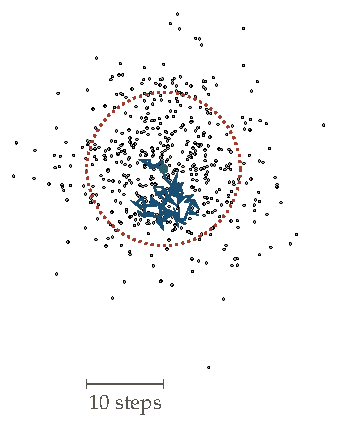
\includegraphics{fig_ch9_random_walk.pdf}
	\caption{End points of $500$ random walks of $100$ unit steps each in the plane (grey dots), all starting at the centre (dark dot). One of the walks is drawn in full (blue). The dotted circle has a radius of $10$ steps.}
	\label{pr:fig:random_walk}
\end{figure}

The same walk is diffusion, Brownian motion, the conduction of heat and the friction inside a gas. In astrophysics it is the slow escape of light from the Sun (Chapter~\ref{ch:radiation}), of neutrinos from a collapsing stellar core, and of cosmic rays from the Galaxy's magnetic field. It gives the $\sqrt N$ law and the flux that flows down any gradient.

\paragraph{The $\sqrt N$ law.} Let a particle take $N$ steps $\vec s_1,\dots,\vec s_N$, each of length $s$ and each in a random direction independent of the others. Its displacement is $\vec R=\sum_i\vec s_i$. Averaging over many walks,
\begin{align}
	\avg{R^2}
	&\eqby{1} \sum_{i=1}^N\sum_{j=1}^N\avg{\vec s_i\cdot\vec s_j} \nonumber\\
	&\eqby{2} \sum_{i=1}^N\avg{s_i^2}+\sum_{i\neq j}\avg{\vec s_i\cdot\vec s_j} \nonumber\\
	&\eqby{3} Ns^2 .
\end{align}
\begin{explain}
	\item $R^2=\vec R\cdot\vec R$, with each $\vec R$ written as its sum of steps.
	\item Split the double sum into the terms with $i=j$ and the rest.
	\item Each step has length $s$. Two different steps point in independent random directions, so their dot product is as often negative as positive and averages to zero. This is the same step that makes the variances of independent noise sources add (Eq.~\eqref{cc:eq:var_add}).
\end{explain}
\begin{equation}
	\boxed{R_{\rm rms}=\sqrt{N}\,s.}
	\label{pr:eq:sqrtN}
\end{equation}
Real free paths vary in length. For the usual exponential spread of free paths with mean $s$, the average of $s_i^2$ is $2s^2$, which changes only the factor in front, not the $\sqrt N$.

To cover a distance $D$ the walk needs $N=(D/s)^2$ steps. At speed $v$ each step takes $s/v$, so the time is
\begin{equation}
	t=N\,\frac sv=\frac{D^2}{s\,v}.
	\label{pr:eq:walk_time}
\end{equation}
The time grows as $D^2$. Twice the distance takes four times as long. Compared with flying straight across, the walk is slower by $D/s$, the number of free paths across the distance.

\paragraph{Flux down a gradient.} Let the number density $n(x)$ of the walkers change along $x$, and look at the particles crossing the plane at $x$. A particle crossing it at an angle $\theta$ to the $x$-axis last scattered, on average, one free path back along its flight, at $x-s\cos\theta$. It therefore brings the density found there. Particles fly in all directions equally, a fraction $d\Omega/4\pi$ of them within a solid angle $d\Omega$, so the net number crossing per unit area per unit time is
\begin{align}
	J
	&\eqby{1} \int\frac{d\Omega}{4\pi}\,v\cos\theta\;n(x-s\cos\theta) \nonumber\\
	&\eqby{2} \int\frac{d\Omega}{4\pi}\,v\cos\theta\left[n(x)-s\cos\theta\,\dv{n}{x}\right] \nonumber\\
	&\eqby{3} -v\,s\,\dv{n}{x}\int\frac{d\Omega}{4\pi}\cos^2\theta \nonumber\\
	&\eqby{4} -\frac13\,v\,s\,\dv{n}{x}.
\end{align}
\begin{explain}
	\item Particles moving at angle $\theta$ cross the plane at the rate $v\cos\theta$ per unit density, positive for those moving toward $+x$.
	\item A Taylor expansion of $n$ over one free path.
	\item $\int\cos\theta\,d\Omega=0$, so the uniform part $n(x)$ carries no net flux.
	\item The average of $\cos^2\theta$ over all directions is $\tfrac13$, as in the pressure integral \eqref{pr:eq:pressure_integral}.
\end{explain}
In three dimensions the same holds along each axis,
\begin{equation}
	\boxed{\vec J=-\frac13\,v\,s\,\nabla n.}
	\label{pr:eq:fick}
\end{equation}
Particles flow from where there are many to where there are few. No force is needed, only random motion and a difference in numbers. The flow is larger when the steps are longer. For photons inside a star, with the energy density $aT^4$ in place of $n$, $v=c$ and the mean free path in place of $s$, this becomes the flow of energy out of the star (Section~\ref{rad:sec:diffusion}).

% ==============================================================================
\section{Compare Two Scales (P6)}
\label{pr:sec:p6}

Chapter~\ref{ch:resolution} decided whether two stars are resolved by comparing their separation with $\lambda/D$ (Eq.~\eqref{eq:rayleigh_criterion_result}). Chapter~\ref{ch:ism} chose between Rayleigh, Mie and geometric scattering by comparing the size of a grain with the wavelength (Table~\ref{tab:scattering_regimes}).

Each time, a single ratio decided which physics mattered. A star has many competing effects at once, and most of them are negligible in any given place. Knowing which ones can be dropped is most of the work.

Think of crossing a road. If you can cross before the car reaches you, you are safe, however fast the car is. If the car arrives first, you are not. Only the ratio of the two times matters, and when it is close to one, small changes decide.

In a gas cloud, sound tries to smooth out a squeeze while gravity tries to deepen it. Whichever acts faster wins. Every regime in astrophysics is chosen in this way. That is principle P6.

The smallest example uses only gravity and density. The constant $G$ has units $\mathrm{m^3\,kg^{-1}\,s^{-2}}$ and a density $\rho$ has units $\mathrm{kg\,m^{-3}}$. Their product $G\rho$ has units $\mathrm{s^{-2}}$, so $(G\rho)^{-1/2}$ is the only time that can be built from them. For the Earth's mean density, $5514\,\mathrm{kg\,m^{-3}}$, it is $27$ minutes. Any process driven by gravity alone must run on a time of this order.

A ratio of exactly this kind appears in fluid mechanics as the Reynolds number and the Mach number, in kinetic theory as the Knudsen number, and in the chapters before this one as the optical depth $\tau$ (Chapters~\ref{ch:photometry} and~\ref{ch:ism}). It gives a quick way to find the right ratio, by its units, and a rule for reading it.

\paragraph{A time from units, checked against Kepler.} The orbit of a satellite that skims the surface of a uniform sphere of density $\rho$ and radius $a$ gives the same time. Kepler's third law, Eq.~\eqref{eq:kepler3}, sets the orbital angular speed to $\sqrt{GM/a^3}$, so the period is
\begin{align}
	\text{period}
	&\eqby{1} 2\pi\sqrt{\frac{a^3}{GM}} \nonumber\\
	&\eqby{2} 2\pi\sqrt{\frac{a^3}{G\,\tfrac43\pi\rho\,a^3}} \nonumber\\
	&= \sqrt{\frac{3\pi}{G\rho}} .
\end{align}
\begin{explain}
	\item Eq.~\eqref{eq:kepler3}, one full turn at the angular speed $\sqrt{GM/a^3}$.
	\item The mass of a uniform sphere, $M=\tfrac43\pi\rho a^3$.
\end{explain}
The radius has dropped out. The period depends on the density alone, and it is $(G\rho)^{-1/2}$ times the number $\sqrt{3\pi}\approx3.1$. For the Earth it is $84$ minutes, the period of a satellite skimming the surface. Real satellites, $400\,\mathrm{km}$ up, take about $92$ minutes. The units had already said that only the number in front could be missing.

\paragraph{Reading a ratio.} A ratio far from one means that one of the two effects can be dropped, and the physics simplifies. A ratio near one means that both matter, and something changes there, often an instability. The ratios that decide the regime in stars and gas are listed in Table~\ref{pr:tab:ratios}, with the place where each is used.

\begin{table}[htbp]
	\centering
	\begin{tabular}{@{}l l l l@{}}
		\toprule
		\textbf{Ratio} & \textbf{Small} & \textbf{Large} & \textbf{Where} \\
		\midrule
		size / mean free path of light & transparent & opaque & Ch.~\ref{ch:radiation} \\
		sound-crossing time / free-fall time & stable & collapses & Sec.~\ref{sg:sec:jeans} \\
		free-fall time / Kelvin–Helmholtz time & slow evolution & -- & Sec.~\ref{sg:sec:freefall} \\
		particle spacing / quantum wavelength & degenerate & classical & Sec.~\ref{st:sec:eos} \\
		pressure of light / pressure of gas & gas holds the star & light holds the star & Ch.~\ref{ch:structure} \\
		luminosity / Eddington luminosity & bound & blown apart & Sec.~\ref{rad:sec:eddington} \\
		$GM/Rc^2$ & Newtonian gravity & general relativity & Ch.~\ref{ch:compact} \\
		\bottomrule
	\end{tabular}
	\caption{Ratios that decide the regime, and where each is used.}
	\label{pr:tab:ratios}
\end{table}

% ==============================================================================
\section{Problem Set: Six Principles}

\subsection{Problem 1: Weight in a Well}
\label{pr:prob:well}

\textbf{Problem Statement}: Model the Earth as a uniform sphere of radius $R=6371\,\mathrm{km}$ with surface gravity $9.81\,\mathrm{m\,s^{-2}}$.
\begin{enumerate}[label=(\alph*)]
	\item Find the gravity at a depth $d$ below the surface, and at a height $h$ above it.
	\item At what height above the surface is gravity as weak as it is $1000\,\mathrm{km}$ below the surface?
\end{enumerate}

\textbf{Essential Ideas}:
\begin{itemize}
	\item Inside, only the mass within radius $r$ pulls (Eq.~\eqref{pr:eq:shell_theorem}), and for uniform density it is $M(r/R)^3$.
	\item Outside, the whole mass pulls as a point at the centre.
\end{itemize}

\textbf{Detailed Solutions}:
\begin{enumerate}[label=(\alph*)]
	\item \textbf{Inside and outside}. With $g_0=GM/R^2$,
	\[
	\boxed{g(R-d)=g_0\left(1-\frac dR\right),\qquad g(R+h)=\frac{g_0}{(1+h/R)^2}.}
	\]
	\item \textbf{Equal gravity}. At $d=1000\,\mathrm{km}$, $g=g_0(1-1000/6371)=0.843\,g_0$. Setting $(1+h/R)^{-2}=0.843$ gives $1+h/R=1.089$.
	\[
	\boxed{h\simeq0.089\,R\simeq570\,\mathrm{km}.}
	\]
	Gravity falls faster going up than going down. Going down, the loss of mass below is partly made up by coming closer to the centre. Going up, nothing makes up for the greater distance.
\end{enumerate}

\subsection{Problem 2: Light Against Gas}
\label{pr:prob:prad}

\textbf{Problem Statement}: Compare the pressure of light with the pressure of gas.
\begin{enumerate}[label=(\alph*)]
	\item In a room at $293\,\mathrm K$ with $n=2.50\times10^{25}\,\mathrm{m^{-3}}$.
	\item At the centre of the Sun, where $\rho=1.5\times10^5\,\mathrm{kg\,m^{-3}}$, $T=1.57\times10^7\,\mathrm K$, and the ionised gas has a mean mass per particle of $0.62\,m_{\rm H}$.
	\item How does the ratio scale with $T$ and $n$?
\end{enumerate}

\textbf{Essential Ideas}:
\begin{itemize}
	\item Gas pressure $nk_BT$ (Eq.~\eqref{pr:eq:ideal_gas}), light pressure $aT^4/3$ (Eq.~\eqref{pr:eq:photon_gas}).
	\item The ratio is a P6 ratio, $aT^3/(3nk_B)$.
\end{itemize}

\textbf{Detailed Solutions}:
\begin{enumerate}[label=(\alph*)]
	\item \textbf{Room}. $P_{\rm gas}=1.01\times10^5\,\mathrm{Pa}$ and $P_{\rm light}=7.566\times10^{-16}\times293^4/3=1.86\times10^{-6}\,\mathrm{Pa}$.
	\[
	\boxed{P_{\rm light}/P_{\rm gas}\simeq1.8\times10^{-11}.}
	\]
	\item \textbf{Centre of the Sun}. $n=\rho/(0.62\,m_{\rm H})=1.45\times10^{32}\,\mathrm{m^{-3}}$, so $P_{\rm gas}=nk_BT=3.1\times10^{16}\,\mathrm{Pa}$. $P_{\rm light}=aT^4/3=1.5\times10^{13}\,\mathrm{Pa}$.
	\[
	\boxed{P_{\rm light}/P_{\rm gas}\simeq5\times10^{-4}.}
	\]
	\item \textbf{Scaling}. $P_{\rm light}/P_{\rm gas}=aT^3/(3nk_B)$ grows as $T^3/n$. Hot, thin gas is held up by light. This is why light matters most in the most massive stars, which are hotter inside but not denser.
\end{enumerate}

\subsection{Problem 3: A Two-Level Atom}
\label{pr:prob:twolevel}

\textbf{Problem Statement}: Collisions move atoms between a ground level $A$ and an excited level $B$ that lies $0.010\,\mathrm{eV}$ higher. Both levels are single states.
\begin{enumerate}[label=(\alph*)]
	\item In gas at $100\,\mathrm K$, what is $N_B/N_A$ in equilibrium?
	\item If the downward rate is $k_{BA}=10^{-3}\,\mathrm{s^{-1}}$, what is the upward rate, and how fast is equilibrium reached?
\end{enumerate}

\textbf{Essential Ideas}:
\begin{itemize}
	\item Detailed balance, Eq.~\eqref{pr:eq:detailed_balance}, fixes the ratio of the two rates.
	\item The relaxation time is $1/(k_{AB}+k_{BA})$, Eq.~\eqref{pr:eq:relax}.
\end{itemize}

\textbf{Detailed Solutions}:
\begin{enumerate}[label=(\alph*)]
	\item \textbf{Populations}. The gap in temperature units is $0.010\,\mathrm{eV}/k_B=116\,\mathrm K$.
	\[
	\boxed{N_B/N_A=e^{-116/100}=0.31.}
	\]
	\item \textbf{Rates}. $k_{AB}=0.31\,k_{BA}=3.1\times10^{-4}\,\mathrm{s^{-1}}$, and the relaxation time is $1/(1.31\times10^{-3}\,\mathrm{s^{-1}})$.
	\[
	\boxed{k_{AB}=3.1\times10^{-4}\,\mathrm{s^{-1}},\qquad\text{relaxation time}\simeq760\,\mathrm s.}
	\]
\end{enumerate}

\subsection{Problem 4: Perfume in Still Air}
\label{pr:prob:perfume}

\textbf{Problem Statement}: Air molecules move at about $v=400\,\mathrm{m\,s^{-1}}$ with a mean free path $s=6.8\times10^{-8}\,\mathrm m$.
\begin{enumerate}[label=(\alph*)]
	\item How long does a perfume molecule take to cross a $3\,\mathrm m$ room by diffusion alone?
	\item How long would it take flying straight?
\end{enumerate}

\textbf{Essential Ideas}:
\begin{itemize}
	\item The random-walk time $D^2/(sv)$, Eq.~\eqref{pr:eq:walk_time}.
	\item The ratio of the two times is $D/s$, a P6 ratio.
\end{itemize}

\textbf{Detailed Solutions}:
\begin{enumerate}[label=(\alph*)]
	\item \textbf{Diffusion}. $t=(3)^2/(6.8\times10^{-8}\times400)\,\mathrm s=3.3\times10^5\,\mathrm s$.
	\[
	\boxed{t\simeq4\ \text{days}.}
	\]
	\item \textbf{Straight flight}. $3/400\,\mathrm s=7.5\,\mathrm{ms}$. The ratio of the two times is $D/s=4.4\times10^7$. In a real room, air currents carry the scent across in minutes, so the bulk motion of the air beats diffusion by far. Inside stars the same competition between carrying energy by motion and by diffusion decides where a star convects (Section~\ref{st:sec:four_equations}).
\end{enumerate}

\subsection{Problem 5: Gravity's Clock}
\label{pr:prob:clock}

\textbf{Problem Statement}: Evaluate $(G\rho)^{-1/2}$ for the Sun (mean density $1410\,\mathrm{kg\,m^{-3}}$) and for a white dwarf (mean density $10^9\,\mathrm{kg\,m^{-3}}$). What does each number say about how quickly the object can respond to a disturbance?

\textbf{Essential Ideas}:
\begin{itemize}
	\item $(G\rho)^{-1/2}$ is the only time made from $G$ and $\rho$ (Section~\ref{pr:sec:p6}).
\end{itemize}

\textbf{Detailed Solutions}:
\[
\boxed{\text{Sun: }(G\rho)^{-1/2}=3.3\times10^3\,\mathrm s\simeq54\,\mathrm{min},\qquad\text{white dwarf: }3.9\,\mathrm s.}
\]
A star responds to a change in its own balance of forces within times of this order. The Sun readjusts within an hour, a white dwarf within seconds. Both are far shorter than the times over which their heat and fuel change, which is why both can be treated as being in balance at every moment (Section~\ref{sg:sec:freefall}).
